%! TEX program = xelatex
\documentclass[tikz]{standalone}
\usepackage[lining]{ebgaramond}
\usepackage[math-style=ISO, bold-style=ISO]{unicode-math}
\setmathfont{Garamond-Math.otf}

\begin{document}
\newcommand{\labhei}{-3.7}

  \begin{tikzpicture}[scale=1, transform shape]
    \node at ( 0.0, 0.20) {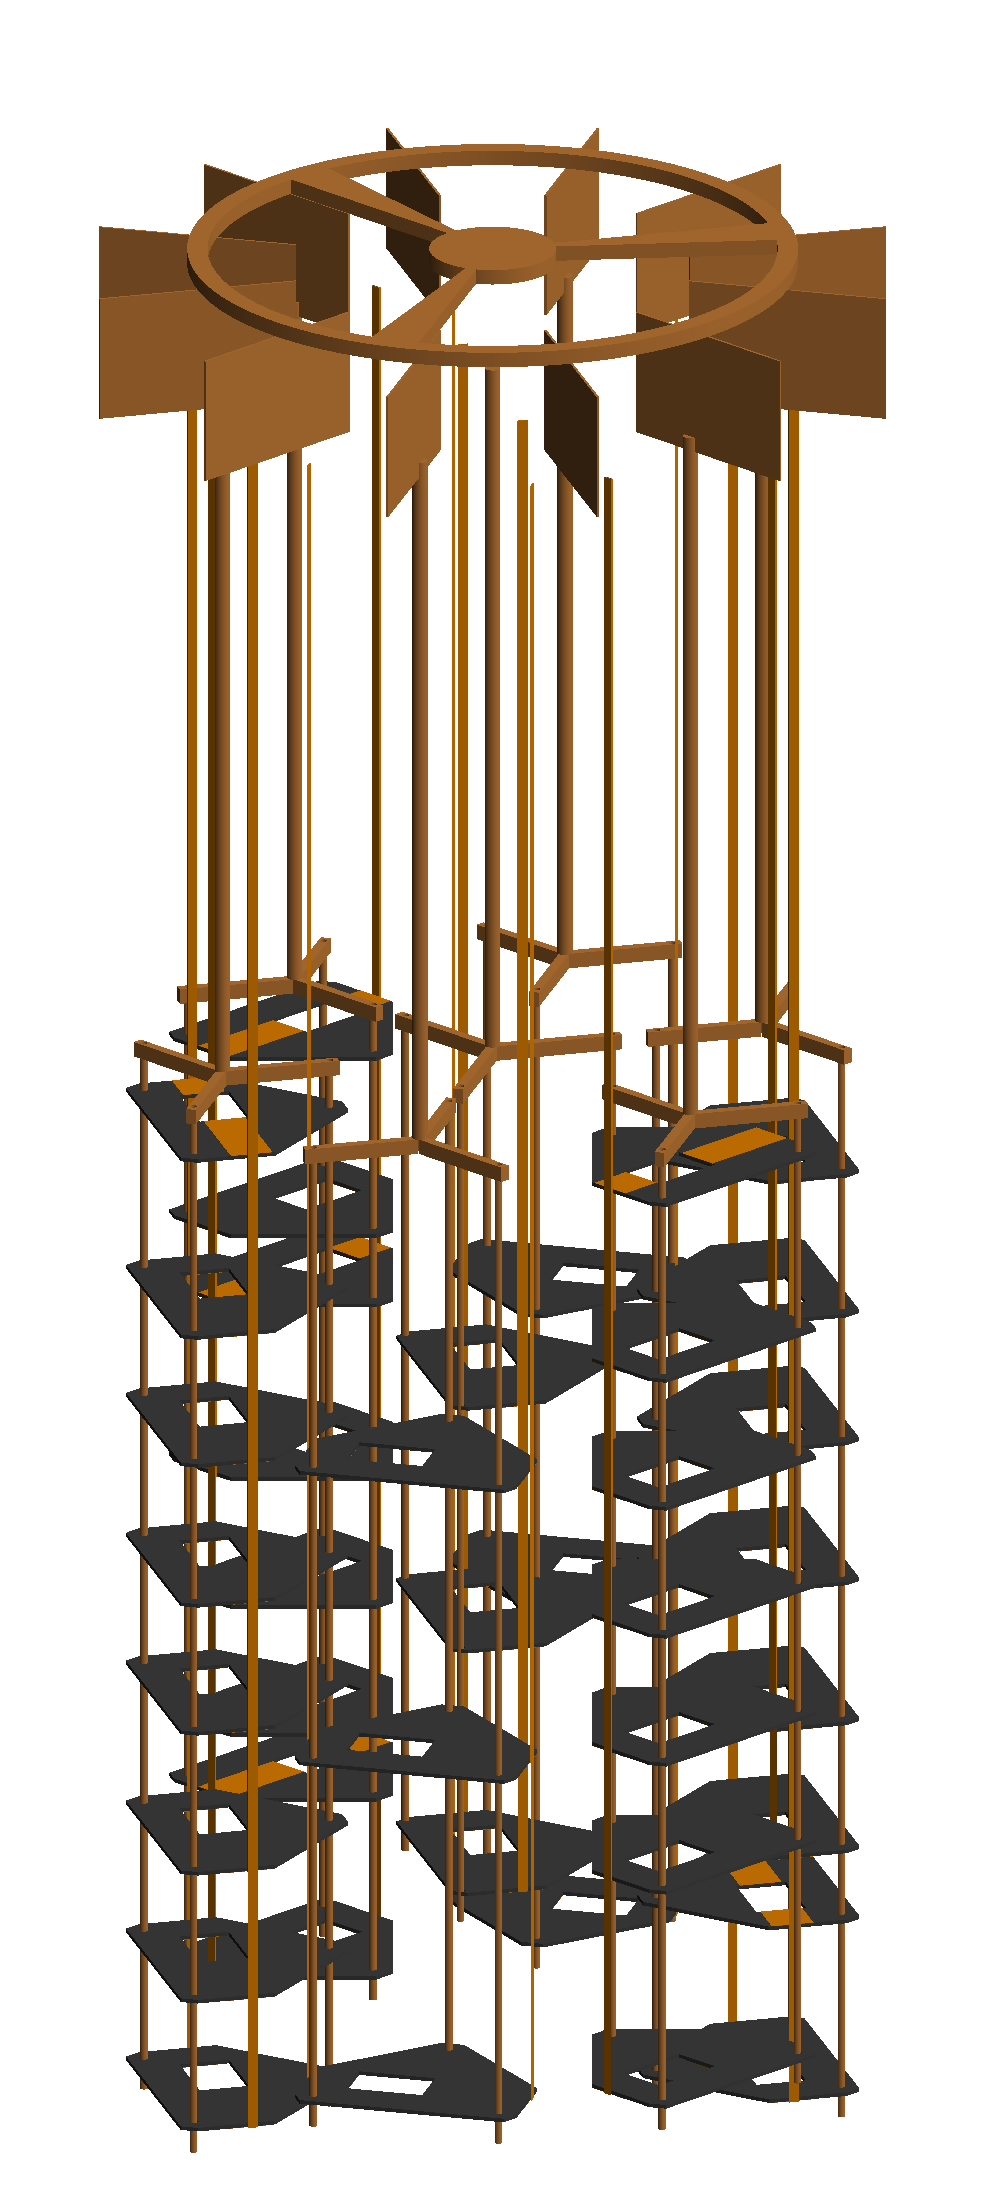
\includegraphics[height=7cm]{mage/draw-array-mounting-ph2.jpeg}};
    \node at ( 3.5, 0.20) {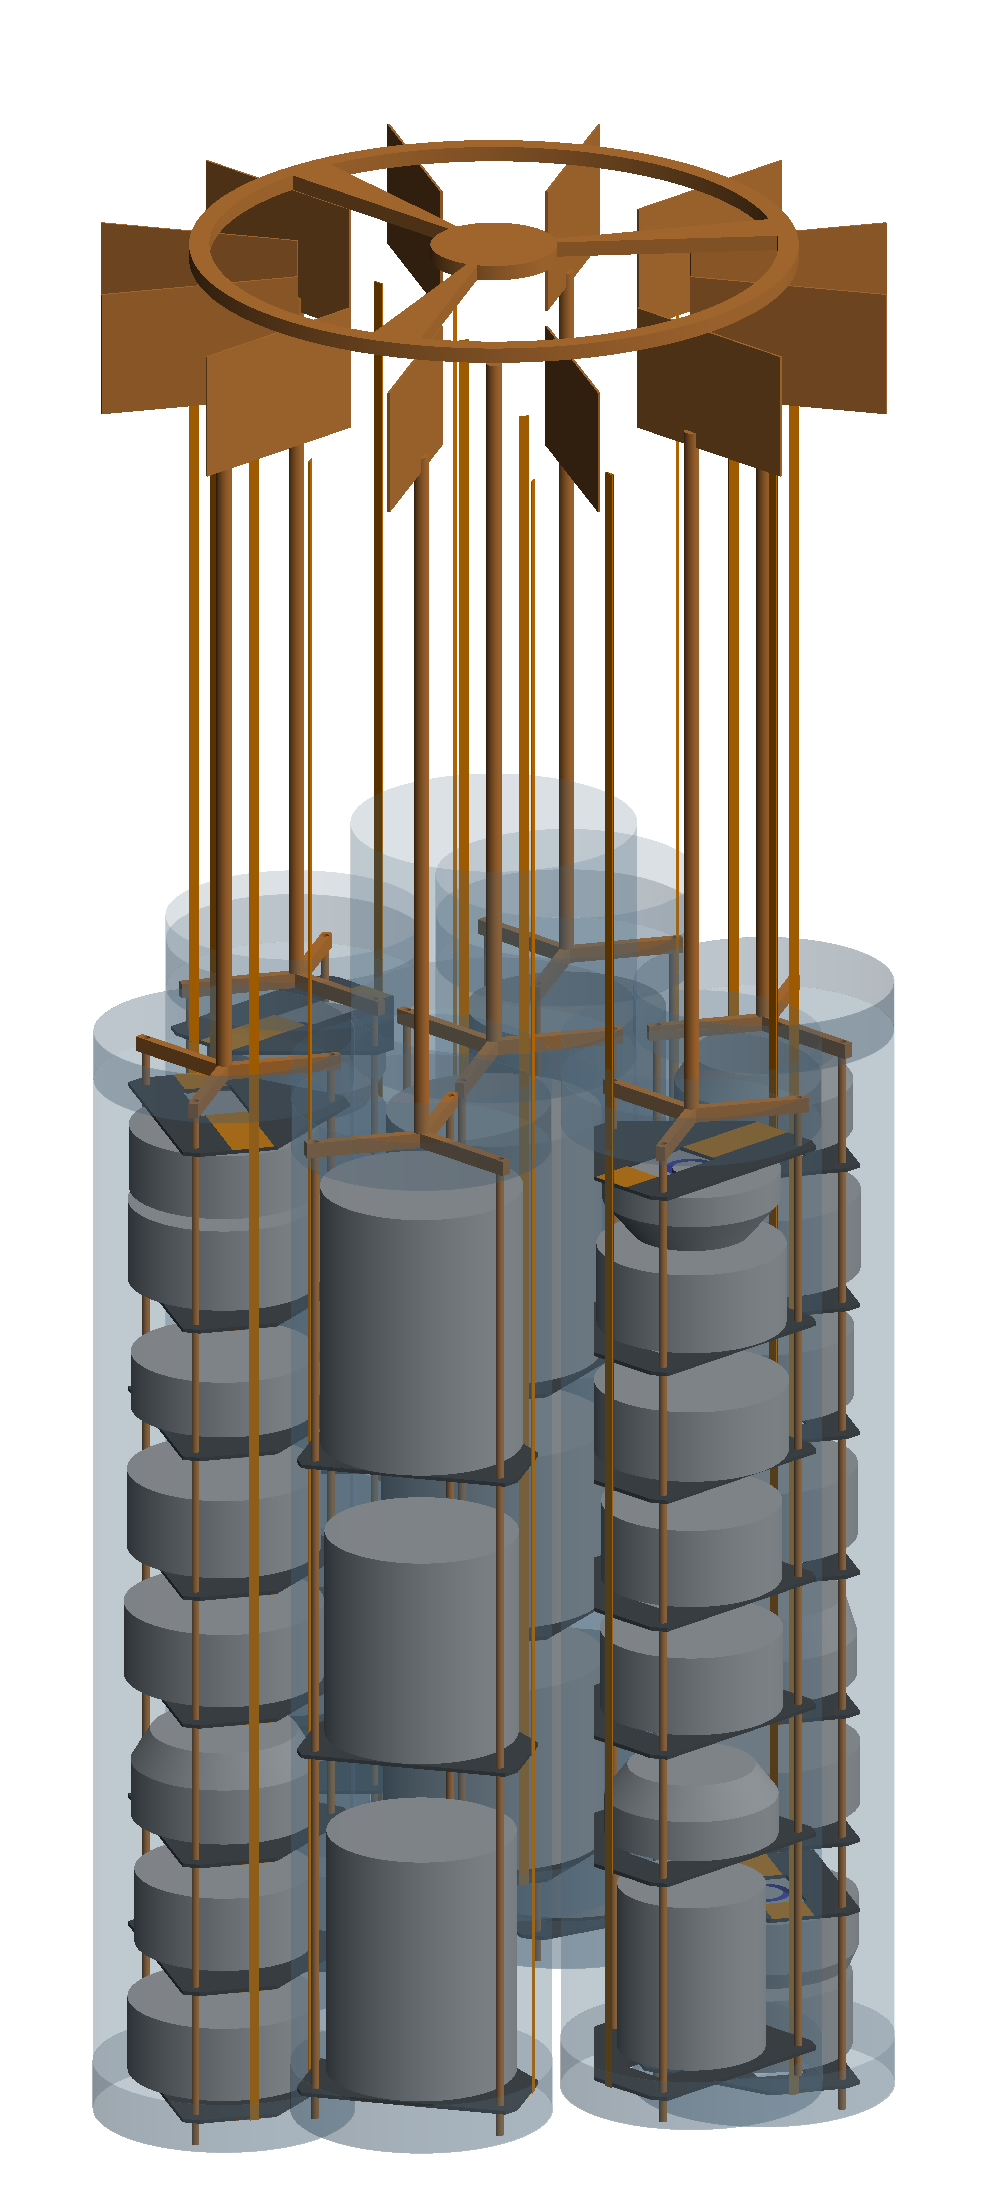
\includegraphics[height=7cm]{mage/draw-array-ph2.jpeg}};
    \node at ( 7.0, 0.20) {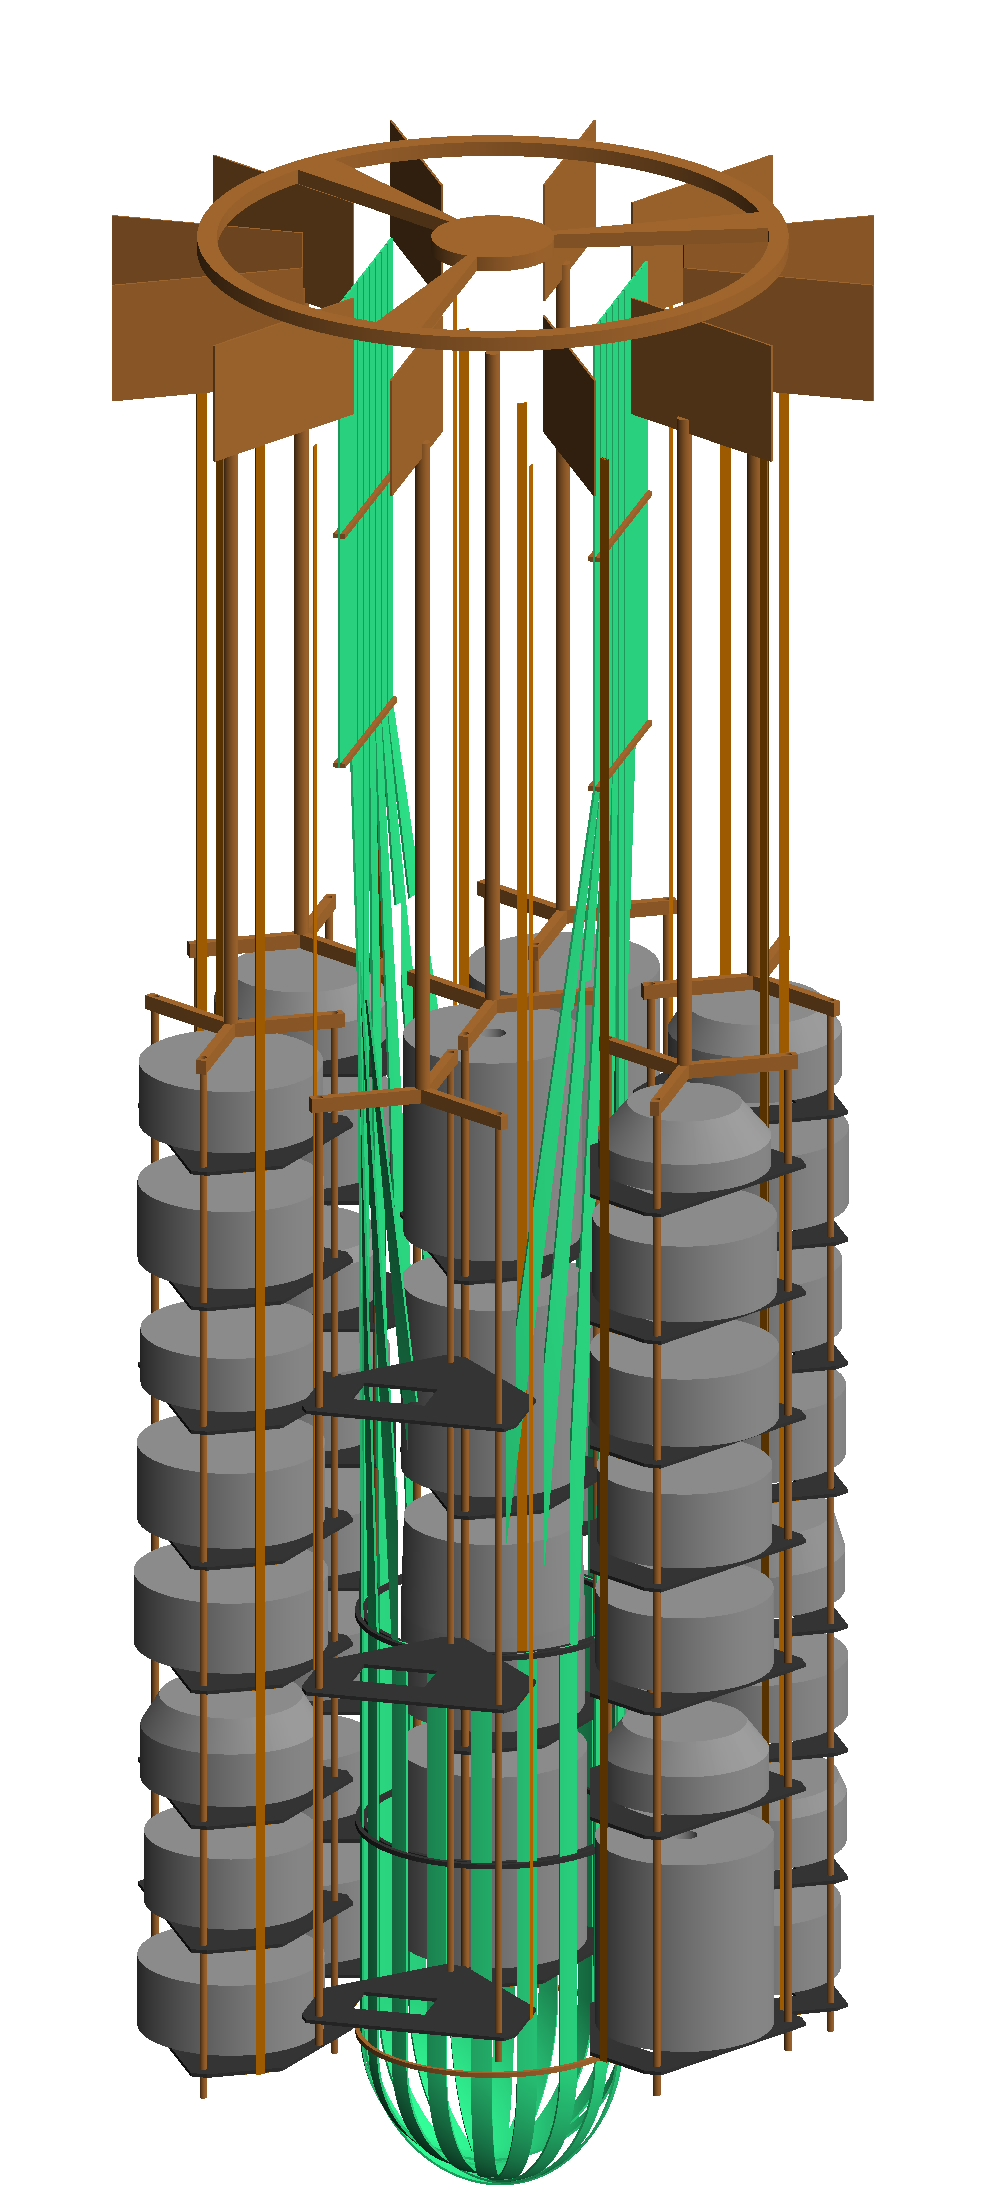
\includegraphics[height=7cm]{mage/draw-array-ph2p.jpeg}};
    \node at (10.4, 0.70) {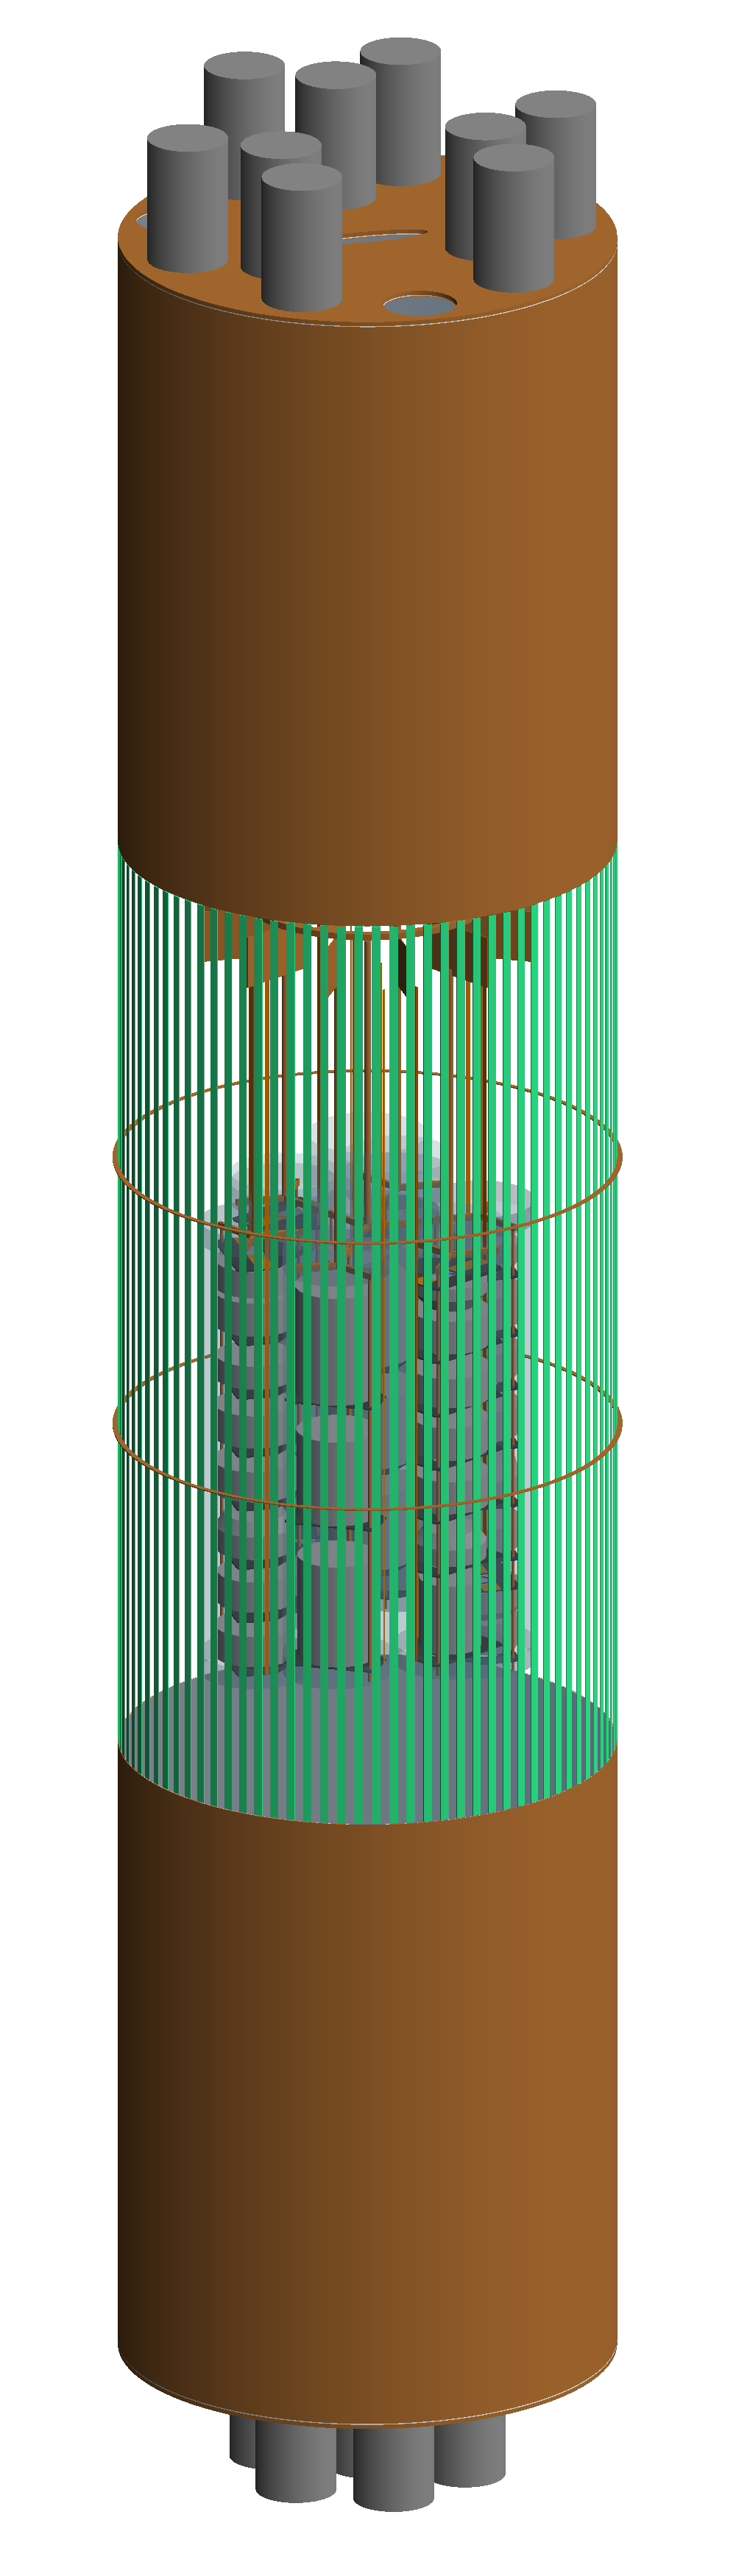
\includegraphics[height=8cm]{mage/draw-larveto-ph2.jpeg}};
    \node at (13.5, 0.70) {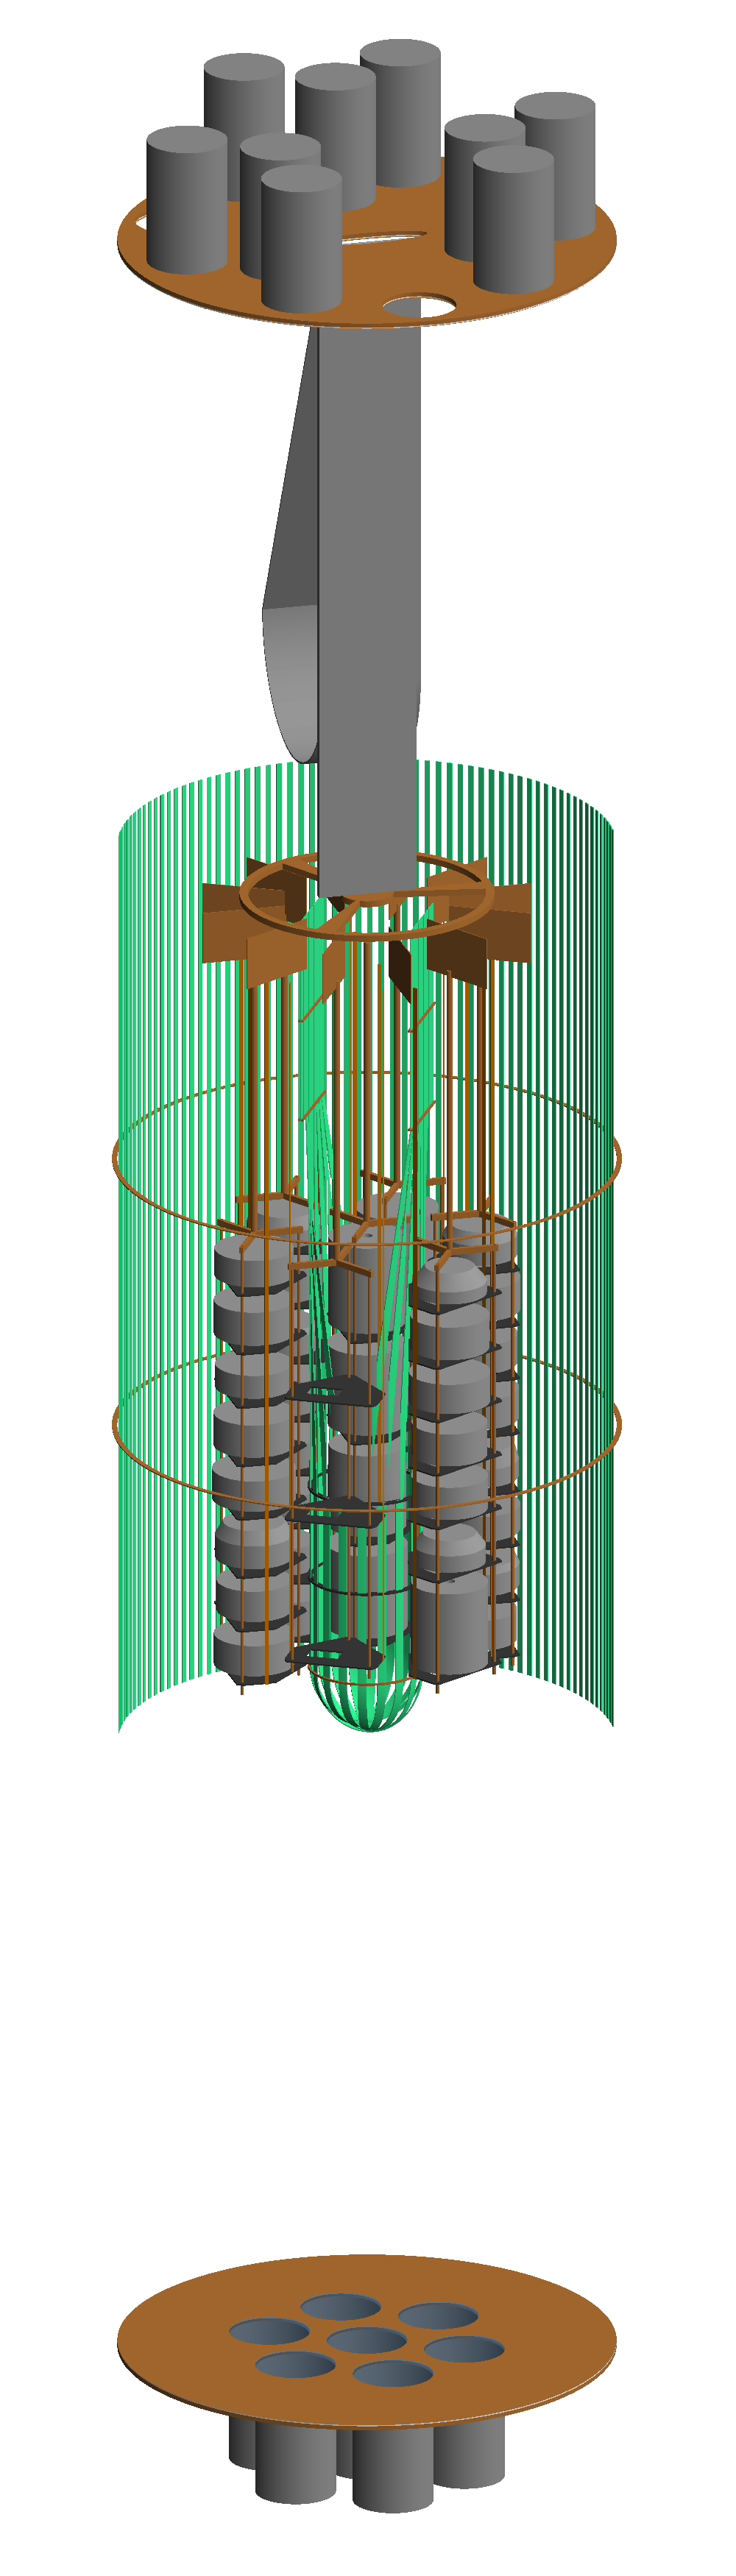
\includegraphics[height=8cm]{mage/draw-larveto-noshroud-ph2p.jpeg}};

    \node at ( 0.0,\labhei) {(a)};
    \node at ( 3.5,\labhei) {(b)};
    \node at ( 7.0,\labhei) {(c)};
    \node at (10.4,\labhei) {(d)};
    \node at (13.5,\labhei) {(e)};
  \end{tikzpicture}
\end{document}
